\documentclass{jfm}

\usepackage{xcolor}
\usepackage{array}
\usepackage{longtable}

\usepackage{graphicx,color}
% \usepackage[section]{placeins}
\usepackage{float}
% \usepackage{graphicx,subfigure}
\usepackage{subcaption}
\usepackage{epstopdf, epsfig}
\usepackage{amstext}
\usepackage{amsmath}
\usepackage{todonotes}
\usepackage{hyperref}
\usepackage{verbatim}
\usepackage{bm}
\usepackage{diagbox}
\usepackage{forloop}

\usepackage{listings}
\usepackage[numbered,framed]{matlab-prettifier}
% \let\ph\mlplaceholder % shorter macro
% \lstMakeShortInline"

\lstset{
  style              = Matlab-editor,
  basicstyle         = \mlttfamily,
  escapechar         = ",
  mlshowsectionrules = true,
}

\newtheorem{theorem}{Theorem}
\newtheorem{defn}{Definition}
\newtheorem{lemma}{Lemma}
\newtheorem{corollary}{Corollary}
\newtheorem{prop}{Proposition}
\newtheorem{assume}{Assumption}
\newtheorem{notation}{Notation}
\DeclareMathOperator*{\argmin}{arg\,min}

\newcommand\nc{\newcommand}
\nc\qu{\quad}
\nc\tends{\rightarrow}
\nc\dint{\int\!\int}
\newcommand{\vect}[1]{\mbox{\boldmath $#1$}}
\nc{\degree}{\mbox{\footnotesize{o}}}

\newcommand{\bes} {\begin{eqnarray*}}
\newcommand{\ees} {\end{eqnarray*}}
\newcommand{\dd} \partial

\newcommand{\non} \nonumber
\newcommand{\ie}{{\it i.e.}\ }
%\newcommand{\eg}{{\it e.g.}\ }
%\newcommand{\etal}{{\it et al.} \ }
\newcommand{\ru}{R_{\rm u}}
\newcommand{\rb}{R_{\rm b}}
\newcommand{\qup}{Q_{\rm u,pore}}
\newcommand{\qbp}{Q_{\rm b,pore}}

\newcommand{\ra}{\rightarrow}

\nc\cA{{\cal{A}}}
\nc\cB{{\cal{B}}}
\nc\cZ{{\cal{Z}}}
\nc\cX{{\cal{X}}}
\nc\cS{{\cal{S}}}
\nc\cR{{\cal{R}}}
\nc\cW{{\cal W}}
\nc\cU{{\cal U}}
\nc\cP{{\cal P}}
\nc\cF{{\cal{F}}}
\nc\cG{{\cal{G}}}
\nc\bz{\bar{z}}
\nc\bZ{\bar{Z}}
\nc\baz{\bar{\zeta}}
\nc\bw{\bar{w}}
\nc\bW{\bar{W}}
\nc\bX{\bar{X}}
\nc\bet{\bar{\eta}}
\nc\bp{\bar{\phi}}
\nc\bP{\bar{\Phi}}
\nc\bc{\bar{\chi}}
\nc\baf{\bar{f}}
\nc\baF{\bar{F}}
\nc\ov{\overline}
\nc\oW{\ov{W}}

\nc\hA{\hat{A}}
\nc\hB{\hat{B}}
\nc\ho{\hat{O}}
\nc\hG{\hat{\Gamma}}
\nc\hS{\hat{S}}
\nc\hO{\hat{\Omega}}
\nc\bO{\ov{\Omega}}
\nc\gham{\hat{\gamma}}
\nc\gcam{\check{\gamma}}
\nc\z{\zeta}
\nc\s{\sigma}
\nc\ep{\epsilon}
\nc\up{\upsilon}
\nc\lam{\lambda}
\nc\sig{\sigma}
\nc\om{\omega}
\nc\kap{\kappa}
\nc\gam{\gamma}
\nc\pa{\partial}
\nc\dom{\pa\Omega}
\nc\domt{\pa\tilde{\Omega}}
\nc\doh{\pa\hat{\Omega}}
\nc\pad[2]{\frac{\pa #1}{\pa #2}}
\nc\padd[2]{\frac{\pa^2 #1}{\pa {#2}^2}}
\nc\pard[3]{\frac{\pa^2 #1}{\pa {#2}\pa {#3}}}
\nc\nd[2]{\frac{d #1}{d #2}}
\nc\ndd[2]{\frac{d^2 #1}{d {#2}^2}}
\nc\ds{\displaystyle}
\nc\del{\nabla}
\nc\lap{\nabla^2}
\nc\ud{|\z|\leq 1}

\nc\capil{\mbox{Ca}}

\nc\pt{\tilde{a}}
\nc\ft{\tilde{f}}
\nc\vt{\tilde{v}}
\nc\wt{\tilde{w}}
\nc\nt{\tilde{\nu}}
\nc\xit{\tilde{\xi}}
\nc\xt{\tilde{x}}
\nc\etat{\tilde{\eta}}
\nc\nht{\tilde{\hat{\eta}}}
\nc\Taut{T}
\nc\zt{\tilde{\z}}
\nc\nut{\tilde{\nu}}

\nc\At{\tilde{\cA}}
\nc\qt{\tilde{B}}
\nc\Ct{\tilde{C}}
\nc\dt{\tilde{D}}
\nc\Dt{\tilde{\cU}}
\nc\Et{\tilde{L}}
\nc\Ft{\tilde{F}}
\nc\Ht{\tilde{H}}
\nc\Kt{\tilde{K}}
\nc\Lt{\tilde{K}}
\nc\Mt{\tilde{M}}
\nc\Nt{\tilde{N}}
\nc\Pt{\tilde{\Phi}}
\nc\Qt{\tilde{Q}}
\nc\Rt{\tilde{R}}
\nc\St{\tilde{\cS}}
\nc\Wt{\tilde{W}}
\nc\cWt{\tilde{\cW}}
\nc\Xt{\tilde{X}}

\nc\vs{\varsigma}
\nc\vp{\varpi}
\nc\ve{\varepsilon}
\nc\vepa{\ve_{\parallel}}
\nc\vepe{\ve_{\perp}}

%\bibliographystyle{elsarticle-num}


%\nc\captionsize{\footnotesize}

\newcommand{\pejman}[1]{\todo[inline,color=green!40]{Pejman: #1}}
\newcommand{\daniel}[1]{\todo[inline,color=yellow!40]{Daniel: #1}}
\newcommand{\michael}[1]{\todo[inline,color=red!40]{Michael: #1}}
\newcommand{\charles}[1]{\todo[inline,color=blue!40]{Charles: #1}}

\newcolumntype{A}[2]{%
    >{\minipage{\dimexpr#1\linewidth-2\tabcolsep-#2\arrayrulewidth\relax}\vspace\tabcolsep}%
    c<{\vspace\tabcolsep\endminipage}}

\newenvironment{lapsetable}[2]{ % n_cols, wid
    \tabular{
        cc
        *{#1}{>{\centering}A{#2}{1.5}}
    }
    \ignorespaces
    }{
    \tabularnewline
    \endtabular\ignorespacesafterend
}
\newenvironment{shortlapsetable}[2]{ % n_cols, wid
    \tabular{
        c
        *{#1}{>{\centering}A{#2}{1.5}}
    }
    \ignorespaces
    }{
    \tabularnewline
    \endtabular\ignorespacesafterend
}

\newcounter{lapse_iter}
\newcommand{\lapse}[9]{ % name, dt, N, dt_display, n_cols, *crop
    \tabularnewline
    #3 & #4
    \forloop{lapse_iter}{1}{\not{\value{lapse_iter} > #5}}{
        &
        \includegraphics[width=\textwidth, trim={#6cm #7cm #8cm #9cm}, clip]{tableFigs/#1/output_#2_#3/\arabic{lapse_iter}.png}
    }
}
\newcommand{\lapseShort}[6]{ % name, n_cols, width, *crop
    \forloop{lapse_iter}{1}{\not{\value{lapse_iter} > #2}}{
        &
        \includegraphics[width=\textwidth, trim={#3cm #4cm #5cm #6cm}, clip]{tableFigs/#1/\arabic{lapse_iter}.png}
    }
}
\newcommand{\scinote}[2]{${#1}\times10^{#2}$}

\shorttitle{Droplets on a wall}
\shortauthor{M. Li et al.}

\title{Droplets on a Wall: Moving Contact Lines with the Immersed Boundary Method}
\author{Michael Y. Li$^{1*}$, Daniel Chin$^{2*}$, Charles Puelz\aff{3}, Pejman Sanaei\aff{4}\corresp{\email{psanaei@nyit.edu}}}
\affiliation{
    \aff{1}
    Courant Institute of Mathematical Sciences, New York University,\\ New York, NY 10012-1110, USA\\
    \aff{2}
    New York University Shanghai,\\ Shanghai, 200120, China\\
    \aff{3}
    Department of Pediatrics, Section of Cardiology, Texas Children's Hospital and Baylor College of Medicine, Houston, TX 77030-????, USA\\
    \aff{4}
    Department of Mathematics, New York Institute of Technology,\\ New York, NY 10023-7692, USA\\
    $^{*}$M. Y. Liu and D. Chin contributed equally to this work.
}

\begin{document}
\maketitle
\begin{abstract}
In this work, we use the Immersed Boundary (IB) method to simulate the movement of 2D liquid droplets hanging on a vertical wall. The simulation requires a moving contact line (MCL) model and a surface tension model that work well with IB. We propose an MCL model that enforces Navier slip on penalty-simulated immersed boundaries. The static and dynamic contact line angle are endogenous instead of prescribed. We use a liquid-gas interface model that is capable of simulating both surface tension force and unbalanced Young's force with one general equation that does not involve estimating local curvature. We also employ a step-wise re-sampling technique to ensure the uniform distribution of the Lagrangian markers that represent the liquid-gas interface and a step-wise interface splicing method to implement droplet coalescence and separation. 
\end{abstract}

\section{Introduction}
Problems involving the two-way coupling between a fluid and some evolving immersed boundaries are often difficult to model analytically. The Immersed Boundary (IB) method is a numerical method that solves the two-way coupling problem with an elegant assumption that the immersed boundaries are massless \citep{peskin1972flow}. IB represents the fluid with a Eulerian velocity field and the immersed boundaries with arrays of linked Lagrangian markers. The fluid advects the markers and the markers exert forces onto the fluid. 

The massless-boundary assumption is suitable for describing thin elastic membranes common to biological contexts, for example, the interaction between blood flow and heart valves \citep{peskin1972flow}. Similarly, the massless-boundaries assumption is appropriate for liquid-gas interfaces. Thus, with a surface tension model, IB is capable of modelling multi-phase fluid flow \citep{surface_tension_review, surface_tension_IB_estimates_curvature, multi_phase_2018, assessment_VOF_vs_IB}. The next challenge is the moving contact line (MCL) problem that emerges when a solid boundary meets with a liquid-gas interface. \cite{MCL_IBM_surfactant} proposes an MCL model that simulates Navier slip with IB, but it is limited to \textit{fixed} solid boundaries. In this work, we simulate Navier slip between a moving liquid-gas interface and an \textit{evolving} immersed solid boundary. Two types of immersed boundaries (liquid-gas interface, solid surface) coexist and are governed by the same IB numerical method. The Navier slip condition is informed by a recent (2018) molecular dynamics (MD) simulation \citep{MD_2018_its_the_bonds}. The resulting simulation scheme, unlike related works that either prescribe the contact angle \citep{curved_solid_DI_IB, muradoglu2010front} or specify marker velocity \citep{manservisi2009variational}, is capable of reaching the \textit{static} contact angle and the \textit{dynamic} contact angle in an endogenous way. 

In addition to the MCL model, we propose a surface tension model with IB. Using IB to simulate surface tension is often classified as a front-tracking method. Most front-tracking methods, including many IB variants, compute the magnitude of surface tension by estimating the local curvature of the interface from about three to six markers \citep{surface_tension_IB_estimates_curvature, multi_phase_2018}, which is susceptible to errors and instability issues if not specifically combated \citep{assessment_VOF_vs_IB}. \cite{surface_tension_still_tangent_applied_to_segment} computes the surface tension using tangent vector subtraction in every Eulerian cell, thus nullifying the need to estimate curvature. \cite{eulerian_tension_lagrangian_advection} uses tangent vector subtraction for every link between adjacent Lagrangian markers, exploiting the advantage of IB. Our method uses tangent vector summation for every Lagrangian marker (instead of every link). The subtle shift in perspective brings an interesting side effect that the unbalanced Young's force at the three-phase intersection is readily computed by the two markers at both ends of a liquid-gas interface. 

We also employ a step-wise re-sampling technique to ensure the uniform distribution of Lagrangian markers in the liquid-gas interface. Finally, we employ a step-wise interface splicing method to implement droplet coalescence and separation. 

We use our methods to simulate 2D droplets moving on a vertical wall. This scenario is based on a real-life case where a vertical catalyst scaffold removes pollutants such as sulfur dioxide (SO2) from industrial exhaust before release into the atmosphere \citep{MPIreport2018}, which is of considerable environmental interest. We measure the spatial and temporal convergence of our methods. We compare simulation results at equilibrium against the analytical solution. We benchmark our methods with several standard test cases. 

\section{Numerical methods} \label{sec:numerical}
We next implement computational fluid dynamics simulations of the flow around droplets using the Immersed Boundary (IB) method in order to extract torque-orientation profiles. The IB method has proven to be a versatile method for such fluid-structure interaction problems since its development almost forty years ago \citep{peskin1972flow,mcqueen1997shared,arthurs1998modeling,lai2000immersed,griffith2009simulating,balboa2011staggered,devendran2012immersed}. The method describes the solid structure with Lagrangian or co-moving coordinates and the fluid with Eulerian or `lab frame' coordinates, where the forces of interaction between the two are communicated locally in a manner consistent with Newton's laws. For the rigid and fixed bodies considered here, we adopt the Penalty Immersed Boundary Method \citep{kim2016penalty}, which introduces a third set of \textit{tether points} that are absolutely fixed in space and represent the desired shape and location of the solid boundary. The boundary points are connected to the tether points via springs, and it is only the boundary points that interact with the fluid. Stiff springs approximate a rigid boundary, at the cost of numerical stiffness but with the benefit of ease of implementation. In practice, accurate results can be achieved with appropriate choices of spring constant, spatial discretization, time-stepping, and other numerical parameters \citep{kim2016penalty}. 

The continuum form of the coupled fluid-solid dynamical equations are:
\begin{align}
% \rho(\cfrac{\partial\bm{u}}{\partial t}+\bm{u}\cdot\nabla\bm{u}) & =-\nabla p+\mu\Delta\bm{u}+\bm{f},\quad
% \nabla\cdot\bm{u}=0, \label{eq:ib1}\\
% \bm{f}(\bm{x},t) & =\int\bm{F}(s,t)\delta(\bm{x}-\bm{X}(s,t))ds, \label{eq:ib2}\\
% \cfrac{\partial\bm{X}}{\partial t}(s,t) & =\int\bm{u}(\bm{x},t)\delta(\bm{x}-\bm{X}(s,t))d\bm{x}, \label{eq:ib3}\\
% \bm{F}(s,t) & =-k(\bm{X}(s,t)-\bm{Z}(s,t)). \label{eq:wallForce}
% The above is the original. The below is my suggestion
\rho(\cfrac{\partial\bm{u}}{\partial t}+\bm{u}\cdot\nabla\bm{u}) & =-\nabla p+\mu\Delta\bm{u}+\bm{f},\quad
\nabla\cdot\bm{u}=0, \label{eq:ib-ns}\\
\bm{f}(\bm{x},t) & = \sum_{n=1}^{3} \left( \int_{0}^{S_n} \bm{F_n}(s,t)\delta(\bm{x}-\bm{X_n}(s,t))ds \right), \label{eq:ib-spread-force}\\
\cfrac{\partial\bm{X_n}}{\partial t}(s,t) & =\int\bm{u}(\bm{x},t)\delta(\bm{x}-\bm{X_n}(s,t))d\bm{x}. \label{eq:ib-advect}
\end{align}
% 2.2 should be a sum of forces experienced by three types of immersed boundaries. each type of immersed boundary is kept track of via a different $s$
%rewrite these eq's: (2.4)->eq:wall; tension force eq:tension; variable density eq:kim?
Here $\rho$ and $\mu$ are the density and viscosity of the fluid; $\boldsymbol{x}$ and $\boldsymbol{X}$ are the Eulerian fluid coordinate and the Lagrangian boundary coordinate; $\boldsymbol{u}(\boldsymbol{x},t)$ and $\boldsymbol{U}(\boldsymbol{X}(s,t),t)$ represent the fluid and solid velocities; $\boldsymbol{f}$ and $\boldsymbol{F}$ are the Eulerian and the Lagrangian force densities; and $\delta$ is a 2D delta function. Equation (\ref{eq:ib-ns}) is the Navier-Stokes equation describing incompressible flow of a viscous fluid. Equation (\ref{eq:ib-spread-force}) describes how force is imparted from the immersed boundaries to the fluid. Equation (\ref{eq:ib-advect}) ensures the immersed boundaries moves with the local flow field, which invokes the no-slip boundary condition. There are three types of immersed boundaries: the wall boundary ($n=1$), the fluid-gas interface boundary ($n=2$), and the variable density markers ($n=3$). They each have an $\boldsymbol{F_n}$ and an $\boldsymbol{X_n}$. The below subsections will describe each type of immersed boundaries and define their forcing scheme $\boldsymbol{F_n}$. $S_n$ is the $s$ range for a given type of boundary. 

We use a global NS solver based on harmonics in the velocity field. The global NS solver uses Fast Fourier Transform to accelerate the computation, at the cost of not being able to handle variable density/viscosity out-of-the-box. 

The timestep is $dt$ seconds. The spatial refinement, $N$, is the number of Eulerian cells in the problem domain along the y axis. The cell diameter, i.e. meshwidth, is $h$ centimeters. Therefore, we always have $N \cdot h = L$ where $L$ is the diameter of the problem domain. 

\subsection{Wall as an Immersed Boundary} \label{subsec:wall}
The main case that motivates our study is simulating liquid droplets moving on a solid, vertical wall. We simulate the wall as an immersed boundary. In this specific case, because the wall is static, it is arguably easier to treat the wall as a boundary condition. However, we want our MCL method to generalize to non-static solid surfaces (for example, subsubsection \ref{subsubsec:letters}), so we treat the wall as an immersed boundary to maximize generality. Each Lagrangian marker of the wall is tethered to its ground-truth location, thus ensuring no flux and no slip. 
\begin{equation}
\bm{F_1}(s,t) = -k_1 \cdot (
    \bm{X_1}(s,t) - \bm{Z}(s,t)
). \label{eq:wall-force}
\end{equation}
Equation (\ref{eq:wall-force}) describes the tether-point construction and the associated spring force on the boundary. $k_1$ is the spring constant associated with the wall. $\boldsymbol{Z}$ is the ground-truth location. At the start of the simulation we usually have $\boldsymbol{X_1} = \boldsymbol{Z}$ (with subsection \ref{subsec:rb} as an exception). 

The above describes a no-slip wall. The wall behaviors are later modified in the MCL model (subsection \ref{subsec:mcl}). 

\subsection{Surface Tension}
We use the integral formulation to model surface tension \citep{surface_tension_review} so each interface marker is pulled by its two neighbors at constant magnitude. In contrast with \cite{surface_tension_still_tangent_applied_to_segment}, our method is entirely in the Lagrangian domain and does not estimate a tangent vector. 
\begin{align}
\bm{\hat{T}}(s,ds,t) & = \cfrac
    {       \bm{X_2}(s+ds,t) - \bm{X_2}(s,t)}
    {\lVert \bm{X_2}(s+ds,t) - \bm{X_2}(s,t) \rVert}, \\
\bm{F_2}(s,t) & = \sigma \cdot (
    \bm{\hat{T}}(s, h,t) + 
    \bm{\hat{T}}(s,-h,t)
). \label{eq:tension}
\end{align}
Here, $\boldsymbol{\hat{T}}(s,ds,t)$ is the unit tangent vector discretized by $ds$. $\sigma$ is the 2D surface tension coefficient. 

To further justify our approach, we underline that the 2D tension energy is proportional to the interface length. If we view that as the sum of all line segments connecting neighboring markers, then an attractive force with constant magnitude is precisely the gradient of the length of one line segment. Apply that to all line segments and each interface marker will be pulled by its two neighbors at constant magnitude. Note that the total force on any one marker is always normal to the interface. 

\begin{figure}
    \centering
    \includegraphics[width=5cm]{figs/young.png}
    \caption{\label{fig:young}
        The same implementation simulates both the Young's force and the tension force. 
    }
\end{figure}
A consequence of this implementation is that the unbalanced Young’s force at the three-phase contact points are correctly simulated as a side effect. As shown in figure \ref{fig:young}, at the three-phase contact point, there is one interface marker that only has one neighbor. The total force on this marker becomes tangent, instead of normal, to the interface. The horizontal component of this force is balanced by the no-flux force provided by the wall. Notice that the sum of the tension force on all markers is exactly the sum of unbalanced Young’s force on the two markers, just inverted in direction. 

\subsection{Moving Contact Line and Navier Slip} \label{subsec:mcl}
The moving contact line (MCL) problem refers to the apparent contradiction that contact lines can move on a no-slip wall. The mechanism of MCL and how to simulate it had been largely a mystery until 1980 \citep{1979_MCL_confusion}. Many numerical methods have tried to model MCL \citep{2014_MCL_review, curved_solid_DI_IB}. A recent study by \cite{its_the_bonds_original} finds that it is the hydrogen bonds that facilitate the no-slip behavior of water on hydrophilic surfaces. Hydrogen bonds are orders of magnitudes stronger compared to internal viscosity, justifying the validity of the no-slip assumption in non-MCL scenarios. In an MCL scenario, the hydrogen bonds do break, allowing slip. The energy dissipation is quantified by a molecular dynamics (MD) simulation \citep{MD_2018_its_the_bonds}. Therefore, it is proper to treat the wall as Navier-slip where there is an MCL. For example, in \cite{MCL_IBM_surfactant}, MCL is simulated with IB by giving Navier slip boundary condition to the fluid solver. However, if the geometry of the solid boundary evolves with time, imposing it onto the fluid will be difficult. This section proposes a method to implement Navier slip on an immersed boundary. 

We propose a friction model similar to the viscous force. The viscous force is the friction between neighboring layers of the fluid, and wall friction is the friction between the wall and the first layer of the fluid.

\begin{align}
f_f & = \min \{ \lVert f_Y \rVert, f_\text{static\_limit} \}
\cdot \left(
    -\cfrac{f_Y}{ \lVert f_Y \rVert }
\right), \\
f_\text{static\_limit} & =
f_\text{no\_slip} + \mu(\theta)
\cdot (
    \bm{u} \cdot \hat{t}
). \label{eq:friction}
\end{align}
where $f_f$ is the resulting wall friction, $f_\text{static\_limit}$ the static friction threshold, $f_Y$ is the local unbalanced Young's force, $f_\text{no\_slip}$ is the minimum friction force (an exogenous parameter that allows partial no slip), $\theta$ is the contact angle, $\mu$ is a function that gives a friction coefficient without unit, and $\hat{t}$ is the unit vector tangent to the wall. 

Function $\mu(\theta)$ computes the friction coefficient given the contact angle. Our implementation of $\mu(\theta)$ is based on a regression of measured results yielded from \cite{MD_2018_its_the_bonds}. 
\begin{lstlisting}[language=Matlab, caption = {Function $\mu$}]
function coef = mu(angle)
  if angle > 1.117
    if angle > 2
      coef = 1.54;
    else
      coef = - 8.48 * angle + 18.5;
    end
  else
    coef = - 19.1 * angle + 30.31;
  end
end
\end{lstlisting}

We believe more accurate results can be obtained from fine-tuning $\mu(\theta)$ based on MD studies such as \cite{MD_navier}. 

The resulting macroscopic behaviors are analogous to static friction and sliding friction. When the contact angle is large enough such that $|f_Y| < f_\text{static\_limit}$, the contact point is non-slip, hence $f_f = -f_Y$, which is identical to the no-slip condition. 

We integrate this friction into IB. Notice that $f_f$ is not directly an IB force; it is an abstract formulation that applies to the continuous reality. To use IB to simulate our MCL model, $f_f$ is reflected in a change of behavior of the wall. Subsection \ref{subsec:wall} describes the penalty method we use to simulate a no-slip wall. To simulate a Navier-slip wall, we use what we call the \textit{incur-redeem-dismiss} penalty method. In this view, the no-slip penalty method would be an \textit{incur-redeem} penalty method. In the no-slip penalty method, as a marker moves away from its initial location, penalty is \textit{incurred}. A penalty force brings it back. The penalty will never be fully \textit{redeemed} until the marker returns to its correct location. This guarantees no flux and no slip. Now we introduce another way penalty can decrease: \textit{dismissal}. No fluid flow is involved. Penalty is instantly decreased within a timestep by displacing the marker. Our MCL model dictates that at each time step every wall marker should have its penalty dismissed until the resulting tether force equals to $f_\text{static\_limit}$. Consequently, the amount of penalty dismissed, multiplied by friction force, gives the work done (or in other words, heat dissipation). The illustration is given in figure \ref{fig:displace}. 
\begin{figure}
    \centering
    \includegraphics[width=5cm]{figs/displace.png}
    \caption{
        Vertical displacement of the marker corresponds to \textit{dismissal} of penalty, thus implementing Navier slip. The horizontal penalty is never dismissed, ensuring no flux. 
    }
    \label{fig:displace}
\end{figure}

\subsection{Step-wise Interface Re-sampling}
Surface tension is always normal to the interface. The absence of a tangential component allows the fluid flow to easily disrupt the distribution of interface markers. To equi-distribute the markers, \cite{lai2008immersed} uses grid redistribution, while \cite{hou1994removing, MCL_IBM_surfactant} apply artificial tangential velocity. Our method is similar to grid distribution, adding markers to wide gaps and removing markers from tight spaces every timestep. See \ref{subsec:resample} for the apparent improvement that this technique brings. This re-sampling technique, however, is very difficult to implement in 3D where the point array becomes a surface mesh.  

\subsection{Interface Splicing} \label{subsec:splice}
\begin{figure}
    \centering
    \includegraphics[width=8cm]{figs/splice.png}
    \caption{
        Among the six interface splicing scenarios, three pairs are reversed in time and three pairs share the same implementation. 
    }
    \label{fig:splice}
\end{figure}
Figure \ref{fig:splice} shows six conceivable scenarios where the interface needs to be spliced: Two droplets merging, one droplet splitting into two, droplet attaching onto the wall, droplet detaching from the wall, droplet splitting at the wall, and droplets merging at the wall. 

There are three pairs of reversed processes and three pairs of scenarios whose implementations are exactly the same. The iso-implementation cases are locally indistinguishable, since we don't care about liquid and gas switching sides. 
\begin{figure}
    \centering
    \includegraphics[width=6cm]{figs/splice_case.png}
    \caption{
        An important condition for splicing to happen is that the two interfaces are approaching. When the distance between four involved markers become small enough, the algorithm alters two links and makes the topological change. 
    }
    \label{fig:splice_zoom}
\end{figure}
To implement splicing, we store the interface markers in circular double linked lists. The linking direction preserves the polarity information: if one follows the links in the positive direction, the liquid will always be on the right. Figure \ref{fig:splice_zoom} illustrates the splicing event. When the distance between two interfaces is smaller than a threshold and the two interfaces are approaching, splice them. In our method, we have two different thresholds, one for interface-interface events ($h$), and the other for interface-wall events ($2.3h$), where $h$ is the meshwidth (i.e. diameter of one Eulerian grid cell). 

The following two timesteps then become a no-splice window. This rule makes splicing events more atomic so that there will not be multiple splicing events competing to accomplish the same macroscopic effect. Computation-wise, a naive algorithm would check every pair of markers at every timestep. This is $O(N^2)$. We check every pair of markers only once in a while and mark anything close together as suspects. At each timestep we only check the suspect markers. This greatly enhances simulation efficiency. The time interval between global checks is dynamic, computed by dividing the minimum interface distance with the maximum marker velocity, multiplied by $1/2$ and some safeguarding constant. More specifically, our implementation involves maintaining a moving window of past extreme velocities and taking the 40\% percentile. 

\subsection{Variable Density}
The liquid phase and and gas phase have different density. The variable density technique proposed by \cite{IBM_variable_density} uses another set of Lagrangian markers to represent density difference. The fluid solver is still global and is not aware of the density difference. The density difference markers are tethered to their Newtonian and massive counterpart with the penalty method, thus correctly simulating gravitational and inertial differences.
\begin{align}
\bm{v}(s,t) & = \cfrac{\partial \bm{Y}(s,t)}{\partial t}, \\
\cfrac{\partial \bm{v}(s,t)}{\partial t} & = \cfrac
    {k_3 \cdot (
        \bm{X_3}(s,t) - \bm{Y}(s,t)
    ) + m g}
    {m}, \\
\bm{F_3}(s,t) & = k_3 \cdot (
    \bm{Y}(s,t) - \bm{X_3}(s,t)
). \label{eq:variable-density}
\end{align}
Here, $\boldsymbol{Y}$ and $\boldsymbol{v}$ are the location and velocity of the Newtonian particles. $m$ is the mass of each particle, and $g$ is the gravitational constant. $k_3$ is the spring constant associated with the variable density method. 

In our simulation we employ \cite{IBM_variable_density}'s variable density method with some modifications. Instead of their five-step update method, we use a coarser, midpoint method. We also set the allowed distance (between a marker and its Newtonian counterpart) to be one tenth the meshwidth ($h/10$). 

%\section{Scaling \& nondimensionalization} \label{sec:scaling}

\section {Test Cases and Results}
We apply our numerical techniques to simulate several test cases in order to check the validity our techniques. The simulation results are presented in this section. 
\subsection {Convergence Tests}
    We conduct several convergence tests where we vary the timestep and the spatial refinement to see how the simulated behaviors converge. 
    \subsubsection {Test 1: Droplet Sliding}
        \begin{figure}
            \centering
            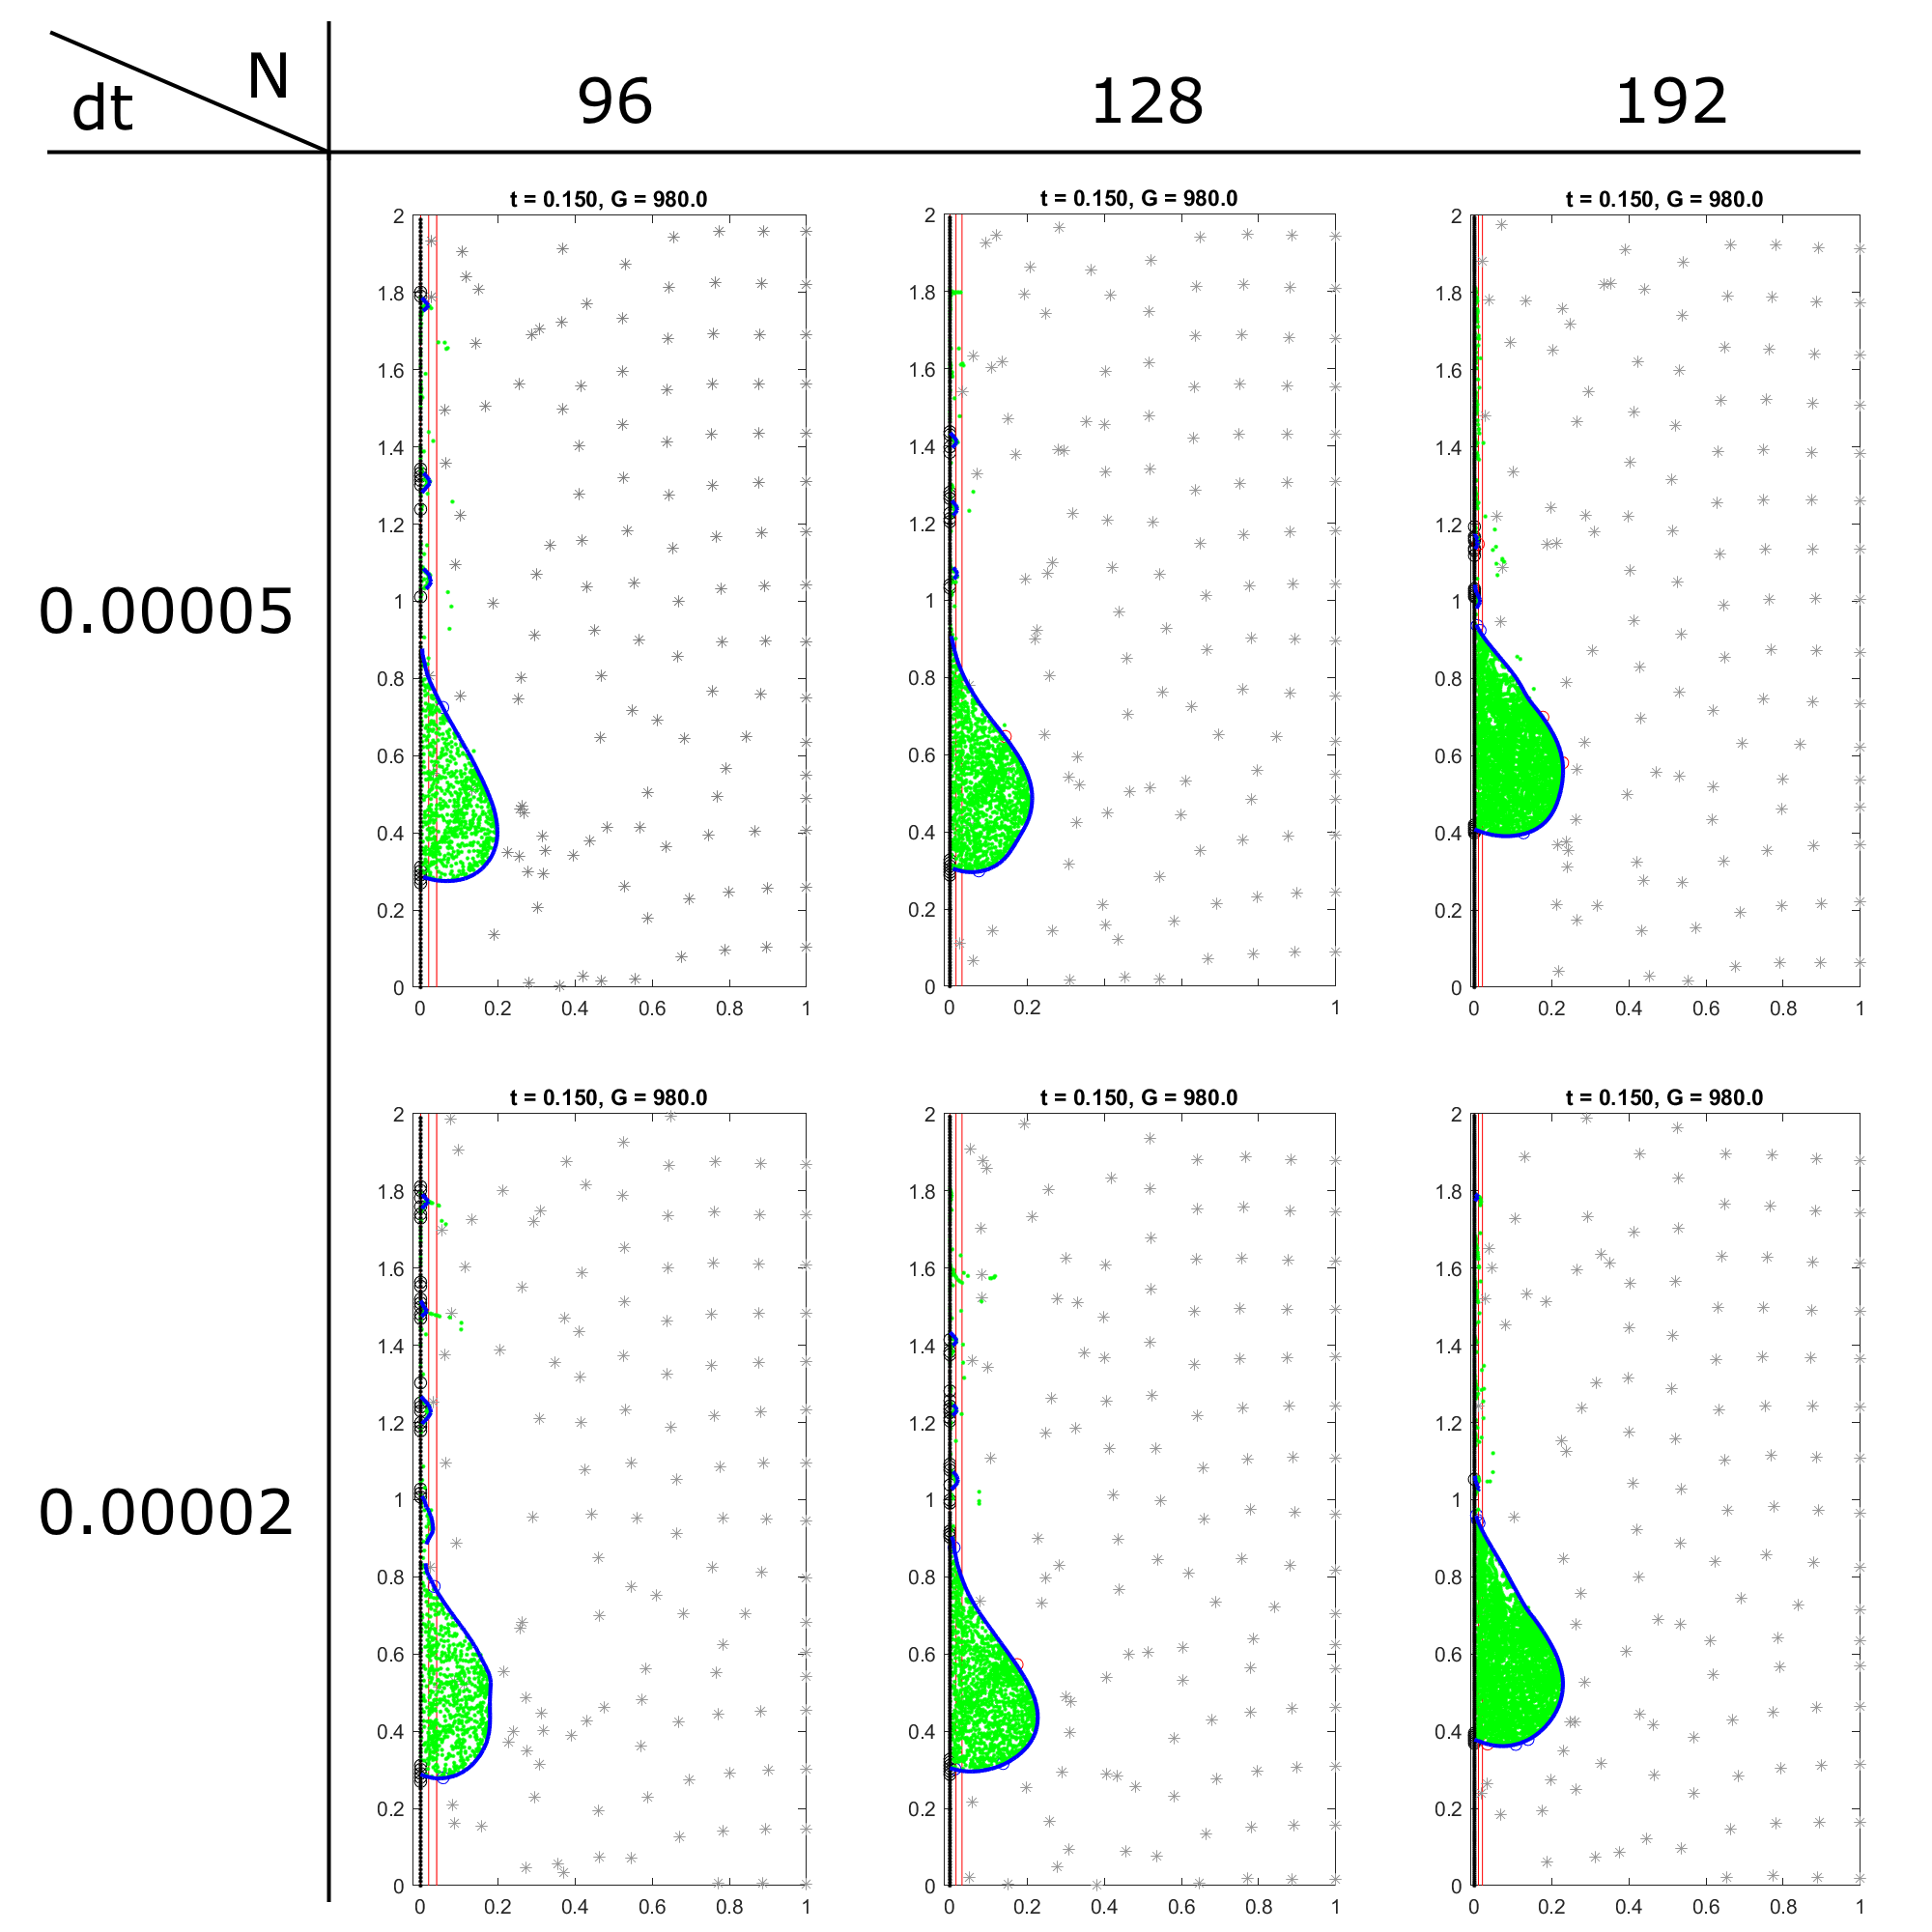
\includegraphics[width=9cm,trim={4cm 6.5cm 4cm 6.5cm},clip]{figs/terminal.pdf} 
            \caption{Terminal state of the sliding droplet experiment, varying $dt$ and $N$. The droplet leaves a trial as it slides down the wall. Convergence is observed near $N = 192$.}
            \label{fig:terminal}
        \end{figure}
        Here we simulate a droplet sliding down a vertical wall and depict the terminal state in the figure \ref{fig:terminal}. In this setup, gravity combats the sliding friction while we vary the timestep and the spatial resolution. We observe that improvement is achieved if we increase the spatial resolution to $192$. Overall, the simulation provides good convergence. 
    \subsubsection {Test 2: Coalescence of Two Droplets}
        \begin{center}
            \begin{lapsetable}{6}{.1}
                $N$ & $dt$ & $t$=0.01&0.02&0.03&0.04&0.05&0.06
                \lapse{merge2}{0.000500}{64} {\scinote{5}{-4}}{6}{5.5}{4}{4.8}{1.5}
                \lapse{merge2}{0.000200}{96} {\scinote{2}{-4}}{6}{5.5}{4}{4.8}{1.5}
                \lapse{merge2}{0.000100}{128}{\scinote{1}{-4}}{6}{5.5}{4}{4.8}{1.5}
            \end{lapsetable}
        \end{center}
        The coalescence of two droplets is an extremely challenging test case since the coalescing moment is very bifurcating. Using our surface tension model and the interface splicing technique, the simulation displays good spatial and temporal convergence. 
    \subsubsection {Test 3: Coalescence of Six Droplets}
        \begin{center}
            \begin{lapsetable}{6}{.13}
                $N$ & $dt$ & $t$=0.01&0.02&0.03&0.04&0.05&0.06
                \lapse{merge6}{0.000200}{96} {\scinote{2}{-4}}{6}{3.4}{3.8}{2.3}{1.5}
                \lapse{merge6}{0.000100}{128}{\scinote{1}{-4}}{6}{3.4}{3.8}{2.3}{1.5}
                \lapse{merge6}{0.000050}{192}{\scinote{5}{-5}}{6}{3.4}{3.8}{2.3}{1.5}
            \end{lapsetable}
        \end{center}
        The six-droplet coalescence test is even more challenging, since the system's response to the first coalescence event is amplified by the successive coalescence events, making the situation chaotic.
        We remark that at $N=128, dt=$\scinote{1}{-4} convergence is already obtained. Our system demonstrates a peculiar property that slightly larger $dt$ leads to instability issues but once instability is solved slightly smaller $dt$ leads to very fast convergence and high accuracy. 
    \subsubsection {Test 4: Letters "IB" Fall into Elastic Pouch}
        \label{subsubsec:letters}
        \begin{center}
            \begin{lapsetable}{7}{.12}
                $N$ & $dt$ & $t$=0&0.03&0.06&0.09&0.12&0.15&0.24
                \lapse{letters}{0.0005}{96} {\scinote{5}{-4}}{7}{6}{4}{5}{5}
                \lapse{letters}{0.0003}{128}{\scinote{3}{-4}}{7}{6}{4}{5}{5}
            \end{lapsetable}
        \end{center}
        This test case demonstrates the capabilities of our method in an all-in-one setting. Note that here the solid membrane is non-static, rendering traditional boundary conditions unsuitable. This shows that our methods are capable of simulating the two-way coupling between a changing-shape solid and a two-phase fluid flow, taking surface tension, Young's force, and solid elasticity into consideration. 

\subsection {Droplets on a Wall}
    In our case setup "droplet on a wall", the problem domain is $1$ cm by $1$ cm. The top and bottom boundary condition is periodic and the left and right boundary condition is symmetric. The flow is incompressible. Liquid density is $1$ g/cm$^2$. Gas density is $0.1$ g/cm$^2$. Viscosity of both liquid and gas is $0.01$ g/s. Surface tension coefficient is $50$ N$\times10^-5$. Gravity is $980$ cm/s$^2$. 
    
    There is a vertical wall at $x=0$. Its minimum static friction $f_\text{min}=25$ N. There is an upward vertical gas flow of $30$ cm/s, prescribed onto the velocity field at $y=0$. The prescribed velocity diminishes as $x$ approaches $0$ in the shape of $tanh$. 
    
    \subsubsection {Study 1: The Effect of Droplet Size}
        \begin{center}
            \begin{shortlapsetable}{6}{.08}
                Diameter & $t$=0&0.02&0.04&0.06&0.08&0.10
                \tabularnewline
                0.4
                \lapseShort{size_effect/output_0.400000}{6}{5}{4}{8.5}{2}
                \tabularnewline
                0.5
                \lapseShort{size_effect/output_0.500000}{6}{5}{4}{8.5}{2}
                \tabularnewline
                0.6
                \lapseShort{size_effect/output_0.600000}{6}{5}{4}{8.5}{2}
            \end{shortlapsetable}
        \end{center}
        Observe that the smaller droplets do not slide down; rather, they obey the "no slip" rule. This aligns with reality and is implemented with the "no slip" term in our MCL model (subsection \ref{subsec:mcl}). 
        
        In the meantime, we tell the program to track the wall markers that \textit{dismisses} any penalty at every timestep. We observe that dismissal only happens near the contact point (usually within 6 to 8 cells). This means that although our MCL model applies to the entire wall, the majority sections of the wall are as though if they were no-slip. This further echos the point made in \ref{subsec:mcl} that the usual assumption, no slip wall, is just a special case in the more general MCL model. 

    \subsubsection {Study 2: Hydro-static Equilibrium}
        We analytically solve the interface shape at hydro-static equilibrium of a droplet hanging on a vertical wall in appendix \ref{app:equi}. 

        The result shows a linear relation between the 2D curvature and the altitude $y$. We run several simulations and compare their equilibrium state against the theoretical results in Figure \ref{fig:h-curvature}. As can be seen, there is an excellent match. However, noise can be observed around the contact points. This is likely due to the insufficient spatial resolution. 
        
        \begin{figure}
        \centering{
            \includegraphics[width=14cm,trim={0mm 0mm 0mm 0mm},clip]{figs/equi.png} 
        }
        \caption{\label{fig:h-curvature} Interface Curvature in Equilibrium.
        \small 
        The analytical solution is shown as the blue line. The orange scattered dots show the curvature observed in the Lagrangian markers. The vertical axis is altitude and the horizontal axis is curvature. From left to right, the gravitational constant $G$ (cm$^2$/s) is gradually increased to alter the droplet shape. The green line highlights the location where curvature is zero. They correspond to the inflection points in the droplet shape. 
        }
        \end{figure}

    \subsubsection {Study 3: Big Droplet Catches Up with Small Droplet}
        \begin{center}
            \begin{shortlapsetable}{8}{.12}
                $t$=&0.01&0.02&0.03&0.04&0.05&0.06&0.07&0.08
                \tabularnewline
                
                \lapseShort{big_chase_small}{8}{5}{4}{8.5}{1.4}
            \end{shortlapsetable}
        \end{center}
        This test case shows the system's response to droplet size in one simulation and, at the same time, demonstrates the interface splicing capabilities near the wall. 
\subsection {Re-sampling Results} \label{subsec:resample}
    \begin{center}
    \begin{shortlapsetable}{3}{.23}
        Re-sample & $t$ = 0.028&0.045&0.078
        \tabularnewline
        Off
        \lapseShort{resample/bad}{3}{7}{4}{8.5}{5}
        \tabularnewline
        On
        \lapseShort{resample/good}{3}{7}{4}{8.5}{5}
    \end{shortlapsetable}
    \end{center}
    Here is a comparison study on the effect of our step-wise re-sampling technique. In the first row, we do not re-sample, resulting in badly distributed Lagrangian markers and, eventually, topological errors. On the second row, adding the re-sampling technique fixes the problem. 

\subsection {Splicing Demos}
    \begin{center}
        \begin{shortlapsetable}{7}{.13}
            $t$=&0.187&0.190&0.193&0.197&0.2&0.103&0.207
            \tabularnewline
            \lapseShort{split}{7}{6.4}{4.2}{4.6}{4.8}
        \end{shortlapsetable}
    \end{center}
    In this demo, a droplet separates into two smaller ones. After the splicing moment, surface tension quickly brings the sharp edge into the body of the droplet. During that process, the surface length of the droplet drastically shrinks, posing a challenge to the interface re-sampling algorithm. Because the edge is sharp, the rapid removal of markers leads to a spurious loss of tension energy. In future works, this can be remedied with an improved interface re-sampling algorithm where the sharpness of edges are checked and blunt areas are prioritized for re-sampling. 
    
    \begin{center}
        \begin{shortlapsetable}{8}{.09}
            $t$=&0.019&0.021&0.022&0.024&0.027&0.029&0.035&0.040
            \tabularnewline
            \lapseShort{wall_merge}{8}{5}{4.8}{9.5}{3.5}
        \end{shortlapsetable}
    \end{center}
    Two droplets coalesce on the wall. This is one of the six basic cases of interface splicing. 
    
\subsection {Rising Bubble} \label{subsec:rb}
    To better benchmark our methods, we refer to a recently proposed multi-phase fluid flow benchmark case \citep{rising_bubble} where a gas bubble rises in a column of liquid. Compared to older benchmark cases, it better amplifies any error in the surface tension simulation, making it more suitable to benchmark multi-phase flow methods \citep{rising_bubble}. Figure \ref{fig:bm_plot} and figure \ref{fig:bm_shape} show our results. 
    
    \begin{figure}
        \centering
        \includegraphics[width=14cm,trim={0mm 0mm 0mm 0mm},clip]{figs/bm_plot.pdf}
        \caption{
            On the left is shown the altitude evolution of the center of mass of the bubble. Of the right is shown the circularity index of the bubble shape. 
        }
        \label{fig:bm_plot}
    \end{figure}
    \begin{figure}
        \centering
        \includegraphics[width=10cm,trim={0mm 0mm 0mm 0mm},clip]{figs/bm_shape.png}
        \caption{
            Benchmarking the bubble shape evolution through time. The error is extremely small. 
        }
        \label{fig:bm_shape}
    \end{figure}

    The two cases proposed in \cite{rising_bubble} both involve variable viscosity. However, our IB method does not handle any variable viscosity. The authors of \cite{rising_bubble} kindly simulated a constant viscosity variant of their test case for us. The details of the case setup can be found in \cite{rising_bubble}. We are using test case 1. Instead of a 1:10 viscosity ratio, our case is a 10:10 viscosity scenario. 
    
    We, again, treat the top boundary as a penalty immersed boundary. Note that the altitude of the ceiling is initialized so that the spring force is already in equilibrium with the fluid gravity. In other words, the ceiling's starting location is slightly below the top boundary. Otherwise, the fluid column would oscillate up and down in the beginning until it reaches the equilibrium. 

% \subsection {Energy and Area Conservation}
%     \daniel{I can track the energy error from interface re-sampling and splicing.}
%     \daniel{Do it!}
%     \daniel{But I did not keep the plotting script QAQ}

% \subsection {Spurious Currents}
%     [compare shrink]
%     \daniel{Do we even include this part? I think Puelz once said this is just well-known for IB methods.}

\subsection {Computation Costs and Instability Issues}
    \begin{figure}
        \begin{subfigure}{.5\textwidth}
        \centering
        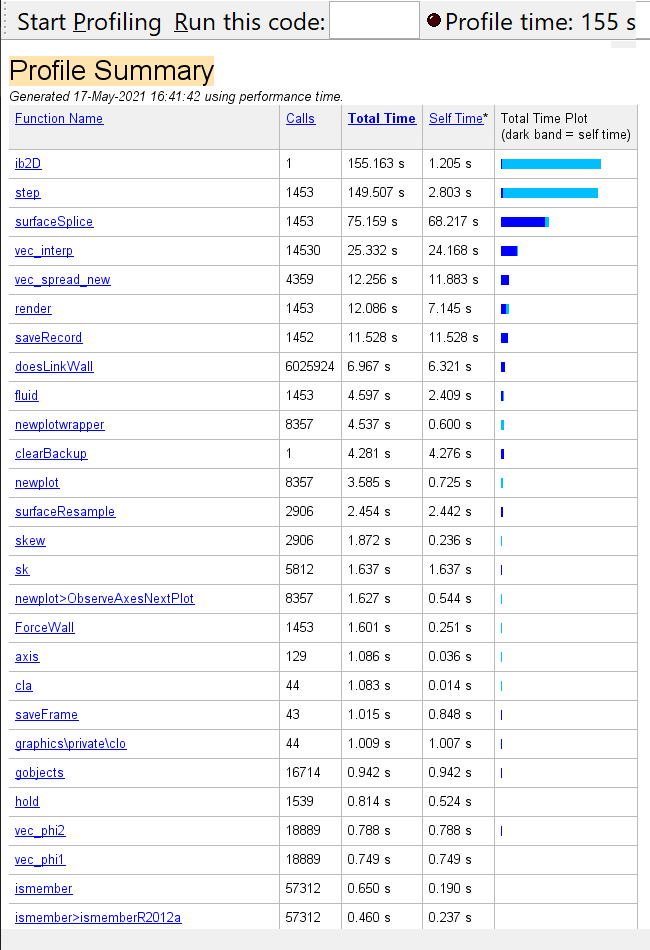
\includegraphics[width=\textwidth,trim={0mm 0mm 0mm 0mm},clip]{figs/time_profiling/summary.png}
        \end{subfigure}
        \begin{subfigure}{.5\textwidth}
        \centering
        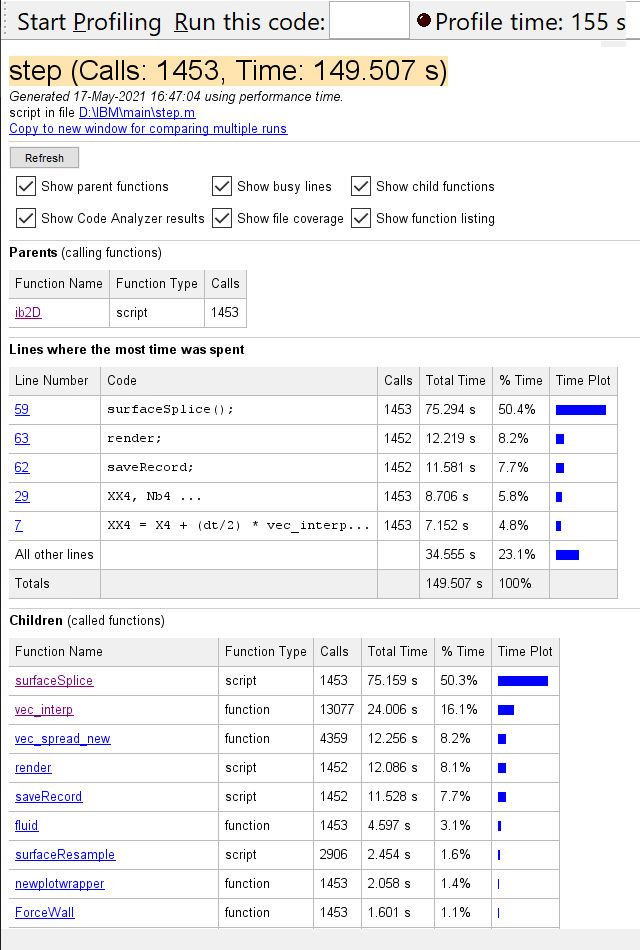
\includegraphics[width=\textwidth,trim={0mm 0mm 0mm 0mm},clip]{figs/time_profiling/step.png}
        \end{subfigure}
        \\
        \begin{subfigure}{.36\textwidth}
        \centering
        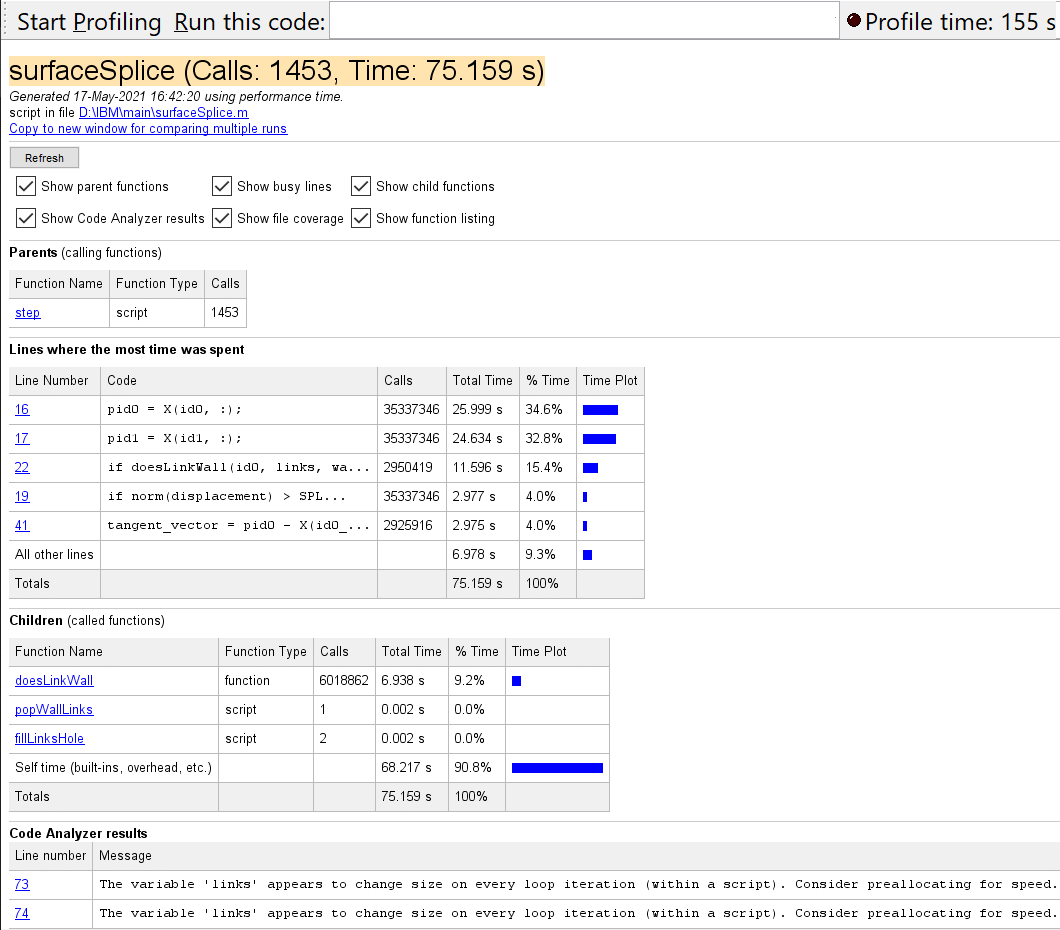
\includegraphics[width=8cm,trim={0mm 0mm 0mm 0mm},clip]{figs/time_profiling/surfaceSplice.png}
        \end{subfigure}
        \begin{subfigure}{.64\textwidth}
        \centering
        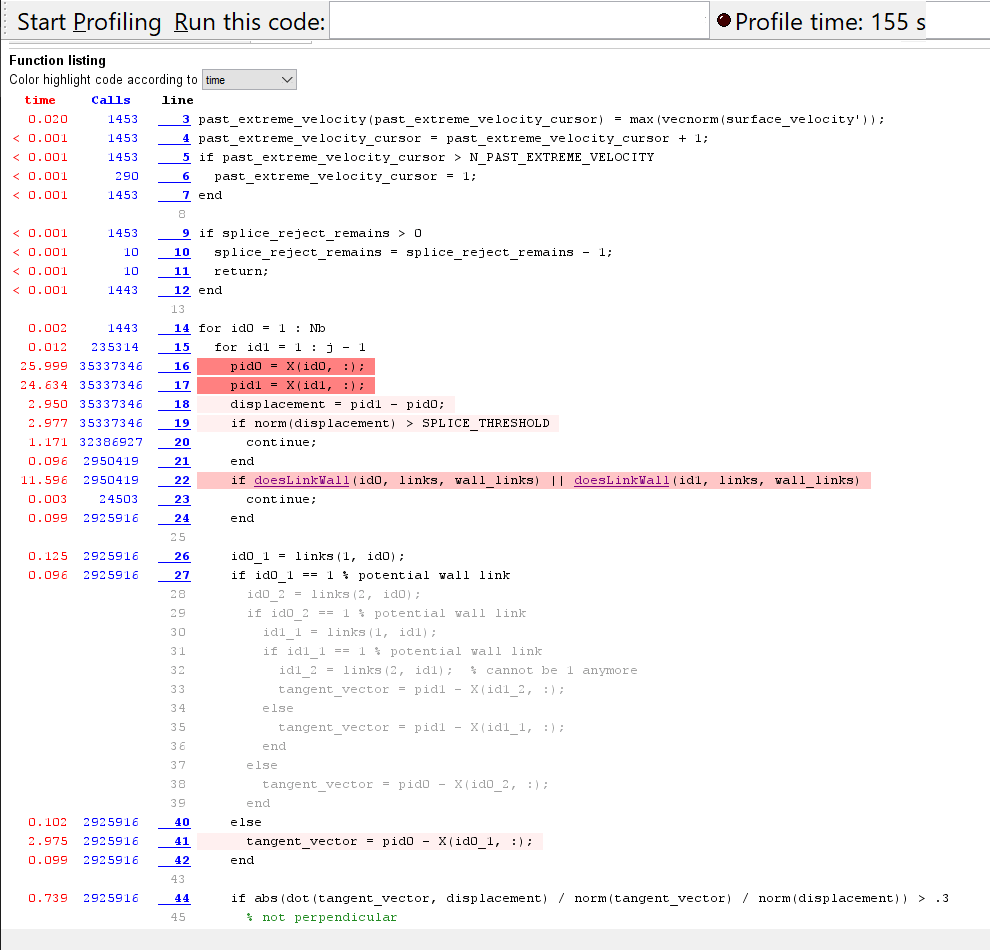
\includegraphics[width=\textwidth,trim={0mm 0mm 0mm 0mm},clip]{figs/time_profiling/code.png}
        \end{subfigure}
        \caption{
            Matlab profiler showing the time consumption at each step of the simulation. Interface splicing is the most expensive computation. 
        }
        \label{fig:computation}
    \end{figure}

    Figure \ref{fig:computation} shows the time consumption of various computations involved in our method. The most expensive computation out of the box is interface splicing. This is due to its $O(N^2)$ nature. Despite the optimization tricks mentioned in \ref{subsec:splice}, it is still the main cost of simulation. The second slowest operation is the vector interpolation for the variable density \citep{IBM_variable_density} markers. Spreading the 2D soup of markers to the Eulerian grid is expensive. The rest of the operations are in the same timescale with the vanilla IB method. 
    
    The existence of surface tension poses a stiffness problem. $dt$ has to be very small to avoid instability. We also observe that, the finer the spatial resolution, the smaller the timestep needs to be. Otherwise, spurious oscillating fluid velocity will emerge and quickly drives everything to NaN. 
    
    The interface re-sampling algorithm makes a minor contribution to the instability. This is intuitive in a sense that removing a marker forces a previously-curving surface to become straight. Although the effect is minimal, it does apply a spurious normal force to the fluid interface. This then encourage the neighboring markers to bend in the other direction, forming a zigzag pattern. In reality, this issue only occurs very rarely. 

\section{Conclusions} \label{sec:conclusion}
Limitations: incompressible. 1:1 viscousity. 
\daniel{Leave till later}

\section*{Acknowledgements} 
We thank Otto Mierka and Stefan Turek for providing the 10:10 viscosity benchmark data. 

\section{Appendices} 
\subsection{Analytical Modelling of the Hanging Droplet Equilibrium} \label{app:equi}
    The shape of the hanging droplet is determined by the following equations:\\
    \begin{equation}
        \vec{g}=g\cdot\hat{j}, \quad
        \nabla{p}=\rho\cdot{g}, \quad
        \frac{\mathrm{d}p}{\mathrm{d}y}=-\rho\cdot{g}, \quad
        p=-\rho\cdot{g}\cdot{y}+p_{\text{const.}}
    \end{equation}
    At the interface, we define the surface tension as:\\
    \begin{equation}
        p=p_{a}+\sigma \cdot \kappa(s),
        \label{eq:pressure}
    \end{equation}
    where $p_{a}$ is the air pressure, and $\kappa(s)$ is the surface curvature. By parametrization of the surface, we get:\\
    \begin{center}
        $r(s)=x(s)\cdot\hat{i}+y(s)\cdot\hat{j}$\\
        $\hat{t}=\frac{\mathrm{d}r}{\mathrm{d}s}=x(s)'\cdot\hat{i}+y(s)'\cdot\hat{j}$
    \end{center}
    We normalize the derivative by writing $1=\left(\frac{\mathrm{d}x}{\mathrm{d}s}\right)^2+\left(\frac{\mathrm{d}y}{\mathrm{d}s}\right)^2$. We get $\left|\frac{\mathrm{d}x}{\mathrm{d}s}\right|=\sqrt{(x')^2+(y')^2}=1$\\
    We define the normal vector as\\
    \begin{center}
        $\hat{n}=\hat{t}\times\hat{k}=y'(s)\hat{i}-x'(s)\hat{j}$
    \end{center}
    Now we have a system of ODEs:\\
    \begin{equation}
    \begin{aligned}
        &\frac{\mathrm{d}\hat{t}}{\mathrm{d}s}=-x\hat{n}(s)\\
        &\frac{\mathrm{d}\hat{n}}{\mathrm{d}s}=x\hat{t}
    \end{aligned}
    \end{equation}
    By some algebra, we get\\
    \begin{center}
        $x''(s)\hat{i}+y''\hat{j}=-x\hat{n}$
    \end{center}
    Multiply both sides by $\hat{n}$, we get\\
    \begin{equation}
        -x=y'x''-x'y''. 
        \label{eq:curvature}
    \end{equation}
    The above equation is the curvature expression for our reparametrization.\\
    Plug \ref{eq:curvature} into \ref{eq:pressure}, we get\\
    \begin{center}
        $p-\rho\cdot{g}\cdot{y(s)}=p_{a}+\sigma(x'y''-y'x'')$\\
        $x'y''-y'x''+\frac{\rho\cdot{g}}{\sigma}y=\frac{\Delta{p}}{\sigma}$
    \end{center}
    Define the capillary length $l=\sqrt{\frac{\sigma}{\rho\cdot{g}}}$,
    and by rescaling, we get\\
    \begin{center}
        $x'y''-y'x''+\frac{u}{l^2}=\frac{\Delta{p}}{\sigma}$
    \end{center}
    Rescaling $x$, $y$ and $s$ in terms of $l$, we get\\
    \begin{center}
        $\bar{x}=\frac{x}{l}$, $\bar{y}=\frac{y}{l}$, $\bar{s}=\frac{s}{l}$, $\Pi=\frac{l\Delta P}{\sigma}$
    \end{center}
    We rewrite the equation in dimensionless form\\
    \begin{equation}
        x'y''-y'x''+y=\Pi
    \end{equation}
    Without loss of generality, set initial conditions $x(0)=y(0)=0$. The first order initial conditions can be described by the contact angle $\theta$: 
    \begin{equation}
        \begin{cases}
            x'(0)=\sin(\theta)\\
            y'(0)=\cos(\theta)
        \end{cases}
    \end{equation}
    
    The above model describes the hydro-static equilibrium shape of a droplet hanging on a vertical wall as a PDE in the Cartesian space. The result shows that there is a linear relationship between the local curvature of the interface and the altitude. 

\bibliographystyle{jfm}
\bibliography{mybibfile}
% \begin{thebibliography}{99}

% \bibitem[Sanaei {\it et al.}(2016)]{Sanaei2016}
% {\sc Sanaei, P., Richardson, G.W., Witelski, T., Cummings, L.J.,}
% Flow and Fouling in a Pleated Membrane Filter.
% {\it J. Fluid Mechanics.} {\bf 795}, 36-59 (2016).

% \bibitem[Sanaei {\it et al.}(2017)]{Sanaei2017}
% {\sc Sanaei, P., Cummings, L.J.,}
% Flow and fouling in membrane filters: Effects of membrane morphology.
% {\it published at J. Fluid Mechanics.} (2017)

% %\bibitem[Sanaei {\it et al.}(2017)]{Sanaei2017cake}
% %{\sc Sanaei, P., Cummings, L.J.,}
% %Optimum Permeability Profile and Fouling in Membrane Filters.
% %{\it Preprint.}

% \end{thebibliography}

\end{document}             % End of document.
